% This is "sig-alternate.tex" V2.0 May 2012
% This file should be compiled with V2.5 of "sig-alternate.cls" May 2012
%
% This example file demonstrates the use of the 'sig-alternate.cls'
% V2.5 LaTeX2e document class file. It is for those submitting
% articles to ACM Conference Proceedings WHO DO NOT WISH TO
% STRICTLY ADHERE TO THE SIGS (PUBS-BOARD-ENDORSED) STYLE.
% The 'sig-alternate.cls' file will produce a similar-looking,
% albeit, 'tighter' paper resulting in, invariably, fewer pages.
%
% ----------------------------------------------------------------------------------------------------------------
% This .tex file (and associated .cls V2.5) produces:
%       1) The Permission Statement
%       2) The Conference (location) Info information
%       3) The Copyright Line with ACM data
%       4) NO page numbers
%
% as against the acm_proc_article-sp.cls file which
% DOES NOT produce 1) thru' 3) above.
%
% Using 'sig-alternate.cls' you have control, however, from within
% the source .tex file, over both the CopyrightYear
% (defaulted to 200X) and the ACM Copyright Data
% (defaulted to X-XXXXX-XX-X/XX/XX).
% e.g.
% \CopyrightYear{2007} will cause 2007 to appear in the copyright line.
% \crdata{0-12345-67-8/90/12} will cause 0-12345-67-8/90/12 to appear in the copyright line.
%
% ---------------------------------------------------------------------------------------------------------------
% This .tex source is an example which *does* use
% the .bib file (from which the .bbl file % is produced).
% REMEMBER HOWEVER: After having produced the .bbl file,
% and prior to final submission, you *NEED* to 'insert'
% your .bbl file into your source .tex file so as to provide
% ONE 'self-contained' source file.
%
% ================= IF YOU HAVE QUESTIONS =======================
% Questions regarding the SIGS styles, SIGS policies and
% procedures, Conferences etc. should be sent to
% Adrienne Griscti (griscti@acm.org)
%
% Technical questions _only_ to
% Gerald Murray (murray@hq.acm.org)
% ===============================================================
%
% For tracking purposes - this is V2.0 - May 2012

\documentclass{sig-alternate}

\usepackage{listings}

\begin{document}
%
% --- Author Metadata here ---
\conferenceinfo{Foss4g Europe}{'14 Bremen, Germany}
% --- End of Author Metadata ---

\title{Comparison of Open Source routing services with OpenStreetMap Data for blind pedestrians}
\subtitle{PgRouting, OpenTripPlanner and OpenSourceRoutingMaschine}

\numberofauthors{3} 

\author{
% 1st. author
\alignauthor Markus Dornhofer\\
       \affaddr{FH JOANNEUM}\\
       \affaddr{Energy and Transportation}\\
       \affaddr{Kapfenberg - Austria}\\
       \email{markus.dornhofer @fh-joanneum.at}
% 2th. author
\alignauthor Werner Bischof\\
       \affaddr{FH JOANNEUM}\\
       \affaddr{Energy and Transportation}\\
       \affaddr{Kapfenberg - Austria}\\
       \email{werner.bischof @fh-joanneum.at}
% 3th. author
\alignauthor Elmar Krajnc\\
       \affaddr{FH JOANNEUM}\\
       \affaddr{Internet Technology}\\
       \affaddr{Kapfenberg - Austria}\\
       \email{elmar.krajnc @fh-joanneum.at}
}

\maketitle

\begin{abstract}
Today's smartphones are more than just a telephone. With built-in positions sensors a phone can be used as a personal navigation device. Even blind or visual impaired people are used to modern phones. With assisted technologies like VoiceOver or Talkback, blind people aren’t reliant on phones with haptic/touchable keys. A lot of effort was made to improve the positioning indoor and outdoors, but affordable technologies are not accurate enough to navigate blind persons on a safe trip. The positioning should be improved by telling the user the surrounding environment. In example the user can verify the position of the sidewalk by telling him the location of the street and the buildings. The goal is the selection of a routing maschine which can deliver a safe route and additional trip information (i.e. crossings with acoustic traffic lights). 
\end{abstract}

\keywords{GIS, Routing, Navigation, Blind, Pedestrian}

\section{Introduction}
For visually impaired and blind people the fastest or the shortest route is not the important fact, they prefer the safest route from a start point to an end point. There are some navigation systems for blind users available on the market, but no system make an highly uses of additional data for blind users. 
OpenStreetMap contains very useful information for visually impaired and blind people. It make it possible to find a safe route from a start point to an end point, which includes acoustical traffic signals and safe sidewalks.Also additional information can improve the navigation. If the user is told that the building is on the right hand side, he/she can verify the information and improve the positioning. Or a warning can occur in front of a waste basket or a traffic sign in an critical position (i.e closed to the head). \\
 
There are many Open Source Routing Systems available today. Many of them focus on car navigation, bicycle navigation and pedestrian navigation. Some of them even include multimodal routing in combination with public transportation systems. In this paper a comparison between different open source routing engines (pgrouting,opentripplanner and open source routing machine) should be made. And how the transfer the technology from car navigation to pedestrian navigation can be done. 
\section{User Requirements}
navigation device should be a smartphone with no additional device
The user interface should be barrier free [Elmar Paper]
How to enter a target address on a smartphone
Less disturbance with the environment
during navigation free hands for the blindman stick an additional stuff
The navigation App should also work in the background

\section{Related Work in blind pedestrian routing and navigation}
The pioneer in free GPS navigation software is Loadstone GPS\cite{loadstone}. It is running on Symbian mobile phones and uses an external bluetooth GPS receiver. The product is very popular in the community of blind and visually impaired people. Nevertheless there is no active development anymore. \\
On the iOS platform Blindsquare\cite{blindsquare} is a very popolar App. It uses point of interest information from foursquare and OpenStreetMap and allow a navigation to the POIs. The actual price is about 24 US Dollar. \\
OsmAnd (OSM Automated Navigation Directions) is a map and navigation application with OpenStreetMap (OSM) data. All map data can be stored on your device's memory card for offline use. Via your device's GPS, OsmAnd offers routing, with optical and voice guidance, for car, bike, and pedestrian. It has a Turn-by-turn voice guidance and does an automatic re-routing whenever you deviate from the route. OsmAnd works well for blind people with Talkback when the uses pre stored favourites. The greatest challenge for the blind people is the destination input, which is only possible with standard keyboard.  \\
'Ready.Set.Access'\cite{weyrer} is a master thesis about intermodal door-to-door application for people with disabilities. The implementation was done with the OpenTripPlanner (section \ref{subsec:otp}) Routing Software. It combines indoor and outdoor navigation. The main focus is on wheelchair accessibility. The project also analyses the topography of a region and flat slops are preferred. In the thesis a geospatial barrier catalogue with six categories (Way Types, Surface Types, Way Related Attribues, Node Information, General Attributes and Public Transport) was one result. \\
Sven Leitinger\cite{sven:osm} from Salzburg Research wrote a guideline to enhance the OSM Data with blind related attributes. He explained most of the OSM tag, which are useful for blind people. The guideline describes the mapping process to record blind related attributes in OpenStreetMap.
The scientific paper\cite{Volkel:2008} Route CheckR focus on route finding for mobility impaired people. A safety factor was embedded in the route calculation. It is recommended to read this paper, if you are interested in safety routing algorithms. The algorithms are not scope of this work.  

\section{OpenStreetMap Data}
OpenSteetMap was founded in the year 2004. In this last 10 years a enormous map material was generated by volunteers. The map data is free available without any licence cost. Therefore a lot of open source routing tools work with OSM data. \\
The map network consist of nodes and ways like a routing graph with special attributes called map features. There are confirmed map features and proposed map features.  Both will be used in the routing process to find the safest route. It is not scope of the project to find new OSM features for blind pedestrians.   

\subsection{Interesting Features for blind people}
Some of the main attributes for blind pedestrians. The information should be given to the users during the navigation.
\begin{itemize}
  \item highway=pedestrian,living\_street,path,footway,steps,elevator
  \item surface=paved,unpaved,asphalt,concrete,concrete:plates, \\ fine\_gravel,metal,paving\_stones
  \item footway=sidewalk,kerb,tactile\_paving
  \item crossing,taffic\_signals:sound  
\end{itemize}

\section{Routing Problem}
The main task of an ordinary routing system is to find the shortest route or the fastest route. In blind person routing also safety plays a important  role. In general those five requirements\cite{weyrer} are needed to do navigation and routing.
\begin{enumerate}
  \item A procedure to set start point and end point
  \item A connected network (routing graph), on which the routing can be performed
  \item An algorithm that computes the route between start point and end point
  \item The inclusion of user requirements in the route computation and selection
  \item The presentation of the results to the use
\end{enumerate}

This work focus most on point 4 of the list. The influence of the user requirements on the route.  

\section{Prerequisites}
Following questions has to be asked to choose the right routing service for the comparison.\\
Is the routing service free of charge and is it possible to adopt it for blind pedestrian routing? What additional information can be in the routing graph? Can it use OpenStreetMap data to generate the routing graph? Can the routing tool be configured to support blind pedestrians? The Web-Frontend is not required for the blind users, but it is important for the developer. It is easier to test different routes and it gives you a good impression about the output of the routing service. 
\section{Comparison between different routing tools}
In a first selection 3 tools has been found, which fulfil the requirements. For sure there are more tools around, but these three are well documented and active.
\begin{itemize}
  \item PgRouting
  \item OpenTripPlanner
  \item OpenSourceRoutingMachine  
\end{itemize}

  
\subsection{Generation of the routing graph}

All routing services in this comparison use OpenStreetMap data to generate the routing graph. It is important that the routing graph has all the OpenStreetMap attributes, which are important for blind people. The process is illustrated in figure \ref{fig:overview}

\begin{figure}
\centering
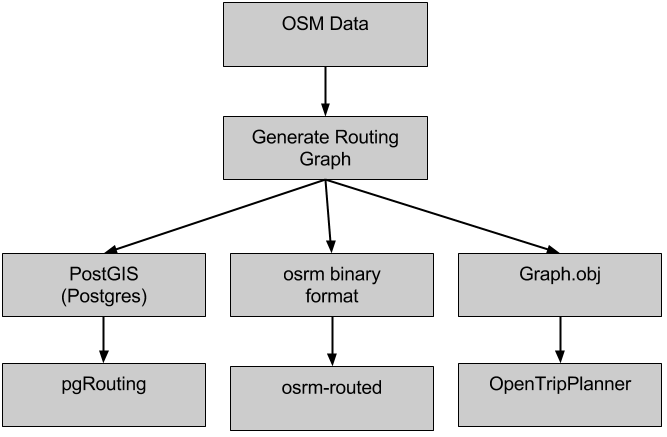
\includegraphics[width=3in]{Overview2.png}
\caption{Overview}
\label{fig:overview}
\end{figure}


\subsection{pgRouting\cite{pgrouting}}
pgRouting is an extension to the PostGIS standard. PostGIS brings spatial information to Postgres database. 
In a workshop the combination of Geoserver and OpenLayers is shown. Also a example with QGIS is included. \\
With some lines of code, it is easy to get a GeoJson track with  some server side programming language (i.e. PHP or Perl). So even interfaces to Smartphone Applications should be manageable. But the lack of turn instructions makes the difference to other software tools.  

\begin{description}
  \item[+] routing network or route can be displayed with GIS software (i.e. QGIS)
  \item[+] many different routing algorithms (Dijkstra, A-Star and Shooting Star)  are implemented
  \item[+] standardised routing graph (POSTGIS)
  \item[-] a lot of components (postgres, postgis, osm2pgrouting, GeoServer, OpenLayers) from different vendors   
  \item[-] difficult to set up the environment 
  \item[-] no turn instructions
  \item[-] no mature Web-Frontend  
\end{description} 


\lstinputlisting[language=Xml,basicstyle=\footnotesize,breaklines=true,frame=lines,caption={osm2pgrouting Mapconfig.xml}]{mapconfig_for_cars.xml}

\subsection{OpenTripPlaner}
\label{subsec:otp}
 
The OpenTripPlaner servlet runs on any standards-compliant Java web server. It is a complete bundle with includes a REST API and a Webfrontend(Figure \ref{fig:otp}). The Webfrontend let you set an start and end point and with button a route can be requested. Drag and Drop the markers as with the OSRM Webfrontend is not possible. The route request takes much more time as with the OSRM routing service. For other Applications like Smartphone Apps there is a well dokumentated REST API, where a route can be requested with many parameters. One routing process can handle multiple profiles (i.e. Walking, Bicycle and Car) and intermodal transportation. GTFS (General Transit Feed Specification) format from Google is used to query the timetables from public transportation companies. 

\begin{description}
  \item[+] includes public transportation ( GTFS)
  \item[+] intermodal (i.e. walk and public transportation) transportaion
  \item[+] well documented REST API
  \item[+] separated JAVA web-apps (Webfrontend and Routing Service)
  \item[+] less dependencies (any standards-compliant Java web server)
  \item[+] multiple profies (Bike, walk, transit) handled by a single routing process
  \item[+] walk speed selectable
  \item[+] safety options in the configure file available
  \item[+] easy to configuration with xml file
  \item[+] Logging and Debugging 
  \item[-] slow route calculation
  \item[-] need much resources to build routing graph   
\end{description} 
 
\begin{figure}
\centering
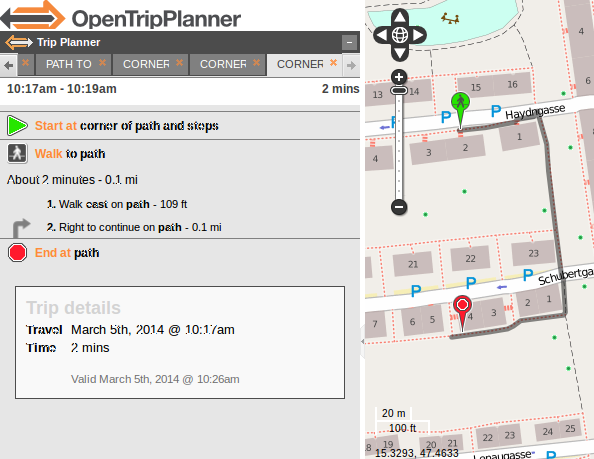
\includegraphics[width=3in]{otp-ss.png}
\caption{Screenshot OTP - Kapfenberg}
\label{fig:otp}
\end{figure}
 
 The graph builder is controlled by an XML configuration. For big regions (i.e. the Country Austria) a lot of RAM is needed. OpenTripPlanner is intended for small and medium geographic areas, but with huge amount of RAM also big areas are possible. The safety parameter was invented for bicycles. There can be a notification, if the osm key surface  has a specific value (i.e. 'Caution: muddy!'). The safe value 1 is default. Very safe streets can have a value below 1 and for dangerous streets can be give a value more than 1. The distance of a street segment will be multiplied with the safe value. I.e. A ten times more dangerous street will have the the length of the street times 10. \\
 With a permission key all transportation types (i.e. Pedestrian, Bicycle, ..) can be put on a white list. So street segment can be accessed by this type of transportation. \\
 It should be possible to convert the bicycle safety features to pedestrian safety features.
 
\lstinputlisting[language=Xml,basicstyle=\footnotesize,breaklines=true,frame=lines,caption={OTP GraphBuilder.xml}]{otp-config.xml}


\subsection{OpenSourceRoutingMachine}
The project is separated in the routing service and a web frontend(Figure \ref{fig:osrm}). The routing service is written in C++ and needs less hardware resources. The routing graph can be influenced by a profile configuration. The profile is a lua script file. So even more sophisticated configurations can be done. In the standard configuration no safety properties are in the profile files. The route can be influenced by the speed parameter, so a safe street can have a higher speed value.  This will also change the travel time. For every profile a single instance of the routing machine is needed.  \\
\begin{description}
\item[+]very fast\cite{luxen-vetter-2011}
\item[+]lua script language to configure the routing graph 
\item[+]shortest path calculation contraction hierarchies, faster then dijskta algorithm
\item[+]blacklist of street, which should not be used
\item[+]delivers Gpx track or turn instruction list in Json,
\item[+]nice Web frontend, supports multiple targets,
\item[-]no safety properties
\end{description}

\begin{figure}
\centering
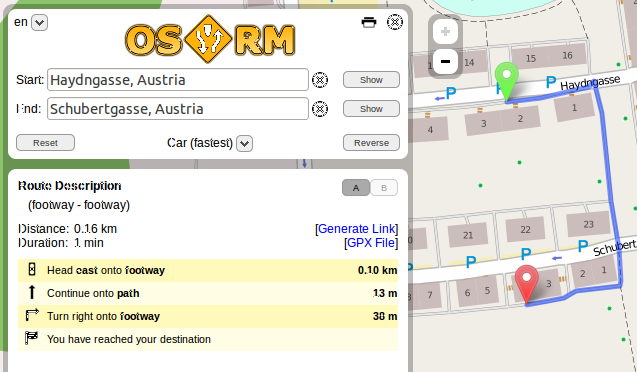
\includegraphics[width=3in]{osrm-ss.png}
\caption{Screenshot OSRM - Kapfenberg}
\label{fig:osrm}
\end{figure}

The route can be configured for blind pedestrians, but there will be no turn instruction if the road name/type stays the same. So even on an orthogonal crossing there can be no turn instruction, if the road stays the same. 
The missing turn instruction can be found on the Figure \ref{fig:osrm}. There is only one turn instructions, instead of two. \\
The route response is well documented. It delivers all track points and for some track points a turn instruction. Some example turn instructions can be found on Table \ref{tab:rlist}. \\ 

\begin{table}
\centering
\caption{Example Routing List}
\begin{tabular}{|c|c|c|c|c|} \hline
No&Turn Angle&Road Name/Type&Distance&Heading\\ \hline
4&282&Werk-VI-Strasse&250m&NW\\ \hline
12&14&Path&24m&SW\\ \hline
\end{tabular}
\label{tab:rlist}
\end{table}

In the profile \ref{lst:osrm} settings different speeds for all kind of roads can be set. Additional OSM meta data can be delivered in the road name field. On every different name a turn instruction is triggered. 


\lstinputlisting[basicstyle=\footnotesize,breaklines=true,frame=lines,caption={OSRM profile.lua},label={lst:osrm}]{foot-osrm.lua}

\section{System Design}
The system was designed as Server/Client Infrastructure. The network graph is held on the server and the routing calculation is also done on the server.  The client ask for the best route with a start point and an destination. Even multiple destination can be handled by the server. Then the server replies with a Json formated file. The json file contains the Gpx Track and turn instructions on specific track points. The turn instructions contain the turn angle, the street name or road type, the distance to the next turn instruction and the heading information (i.e. North West).A network connection is needed for every route request. 

\section{First Results and Tests}
The Android App development started in the same time as the comparison between the routing machines. It was clear that the Application request a route with a start and a stop position and the server replies with a well structured (i.e. XML or JSON) format. \\
The user interface and the navigation instructions are much more important on the smartphone. The routing server should be replaceable. 
By the way a OSRM Routing Service was chosen for the first test. On the Application side a target position can be selected from a list and the actual position was used as start position. After the routing request, the response is displayed in a new list (figure ~\ref{fig:app}). \\
The user can explore the whole trip on the screen. Turn instruction by turn instruction. The distance to the next crossing is spoken periodically. If the proximity of the crossing point was reached the turn instruction was told. \\


 

\begin{figure}
\centering
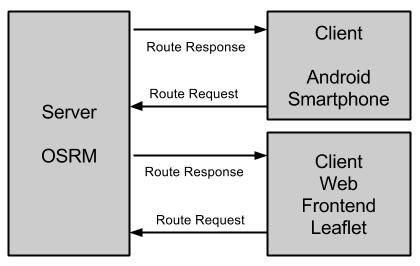
\includegraphics[width=3in]{System-Design2.png}
\caption{System Design}
\end{figure}

\begin{figure}
\centering
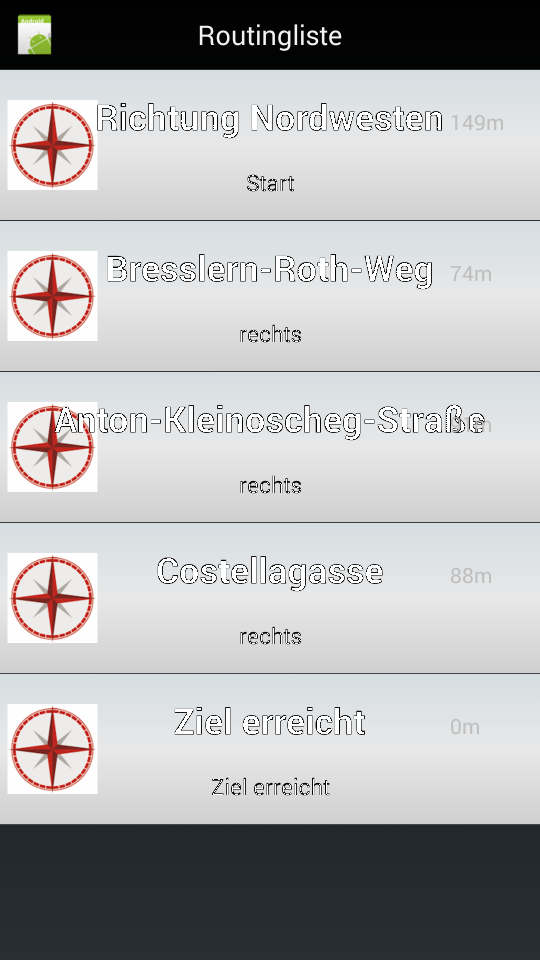
\includegraphics[width=3in]{App2.png}
\caption{Android App}
\label{fig:app}
\end{figure}


\section{Conclusion}



\section{Future work}
The first version was just a prove of concept. The main focus was on the user interface and on a stable server and client communication. The navigation has to be  improved a lot. There has to be a mode where blind people can follow a track in a park without much kerbs. Also a module is needed to get information about the near environment (i.e. Position of the road or building. This information could not be found in the route. There have to be turn instructions where the road stays the same, but makes a curve (i.e. priority roads). \\
Side walks and Streets are closed to each other. It is important that the starting point do not snap to the Street in front the Side walk. \\
And an Evaluation of the priority of footways has to be done. 


\section{Acknowledgements}
The overall project manager is the University of Applied Sciences FH-JOANNEUM in Kapfenberg, Austria. One focus of the project ways4all is to support visually impaired and blind people in their daily lives with the help of usual smartphones. Additional equipment is a no goal of the project. One module focus on indoor and outdoor navigation. \\
Project participants are: Wiener Linien, OEBB and four blind and handicapped organisations. The project is subsidized by the Austrian Federal Ministry
for Transport, Innovation and Technology (BMVIT) and the
Austrian Research Promotion Agency (FFG).

%
% The following two commands are all you need in the
% initial runs of your .tex file to
% produce the bibliography for the citations in your paper.
\bibliographystyle{abbrv}
\bibliography{sigproc}  % sigproc.bib is the name of the Bibliography in this case
% You must have a proper ".bib" file
%  and remember to run:
% latex bibtex latex latex
% to resolve all references
%
% ACM needs 'a single self-contained file'!
%
%APPENDICES are optional
%\balancecolumns

\end{document}
